\documentclass[10pt, a4paper,twoside]{scrartcl}

\usepackage{amsmath}
\usepackage{amssymb}
\usepackage{graphicx}
\usepackage{subcaption}
\usepackage{float}
\usepackage[top=2cm,bottom=3cm,outer=2cm,inner=3cm]{geometry}\usepackage[utf8]{inputenc}
\usepackage{hyperref}
\usepackage[multiple]{footmisc}
\usepackage{parskip}
\usepackage{wrapfig}
\usepackage{xfrac}
\usepackage{xcolor}
\usepackage{tikz}
\usetikzlibrary{arrows}
\usetikzlibrary{arrows.meta}
\usepackage{longtable}
\usepackage{pdfpages}
\usepackage[tikz]{bclogo}
\usepackage{eurosym}

\hypersetup{
    colorlinks=true,
    linkcolor=blue,
    filecolor=magenta,      
    urlcolor=cyan
}

\restylefloat{table}

\newcommand{\warn}[1]{\textbf{#1}}
\newcommand{\con}[1]{\texttt{#1}}
\newcommand{\dis}[1]{\textbf{\texttt{#1}}}

\newenvironment{remember}{\begin{bclogo}[couleur=blue!30,arrondi=.1,logo=\bccrayon,ombre=true]{Remember}}{\end{bclogo}}   
\newenvironment{remark}{\begin{bclogo}[couleur=blue!30,arrondi=.1,logo=\bcinfo,ombre=true]{Remark}}{\end{bclogo}}   
\newenvironment{warning}{\begin{bclogo}[couleur=red!30,arrondi=.1,logo=\bcattention,ombre=true]{Warning}}{\end{bclogo}}   


\title{QRP Automatic Antenna Tuner}
\subtitle{Board rev. 0, Firmware rev. 0.1}
\author{Hannes Matuschek -- DM3MAT\\\texttt{<dm3mat [at] darc [dot] de>}\\\texttt{https://dm3mat.darc.de/atu}}
\date{\today}

\begin{document}
\maketitle

\begin{abstract}
This document describes the first revision of my QRP Automatic Antenna Tuner (ATU). This revision primarily acts as a development platform for the circuit and tuning algorithm. Hence, it lacks some features that are planned for the final revision. Including the build-in battery and charging circuit as well as a reduced power consumption by means of bi-stable relays. To this end, this revision is quiet limited for portable use. 
\end{abstract}
\thispagestyle{empty}
\vfill
\begin{center}
 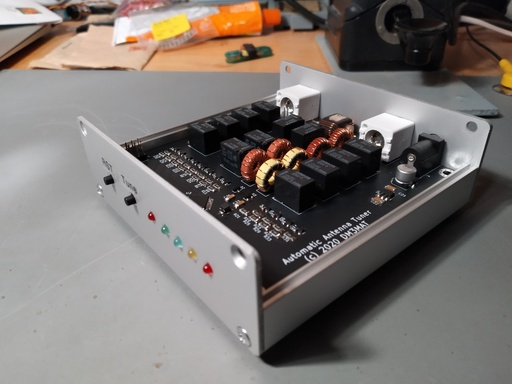
\includegraphics[width=0.7\linewidth]{fig/atu_rev0_small.png}
\end{center}



\clearpage
\tableofcontents
\thispagestyle{empty}

\clearpage
\section{Background}
\begin{wrapfigure}{o}{.5\linewidth}
 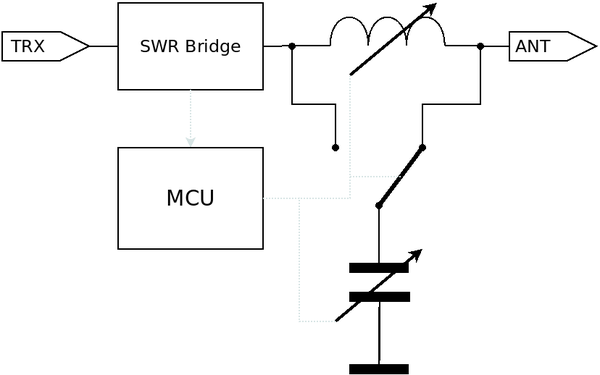
\includegraphics[width=\linewidth]{fig/diagram.png}
 \caption{Basic principle of almost all ATUs.} \label{fig:principle}
\end{wrapfigure}

The basic principle of most ATUs is quiet simple. A micro-controller (MCU) uses an SWR bridge to measure the current VSWR. The MCU then configures a simple L-match to minimize the measured VSWR. This principle is also shown in figure 
\ref{fig:principle}. 

Although there are some ATUs that tune this L-match by actually tune variable capacitors and inductors using motors, the majority of ATUs use relays to \emph{configure} this L-match by \emph{choosing} the required capacitors or inductors. Additionally, these L-match based ATUs usually allow for switching the capacities to the antenna or transceiver side. This allows to also match loads that have an impedance of less than $50\,\Omega$. 

The most expensive BOM parts are the relays. Hence one tries to minimize the number of relays needed. To achieve the maximal tuning range and resolution while minimizing the number of relays needed, a power-of-two series of fixed values of capacities and inductances is chosen. For example: Typical choice of capacities are 10pF, 22pF, 47pF 100pF and finally 220pF. This choice allows to \emph{configure} (almost) any value between 0pF and 400pF with a resolution of about 10pF, using only five relays.

\subsection{L-match Principle}
To explain how an L-match actually tunes a mismatched antenna, one has to understand how a matched and unmatched antenna looks like to a transceiver. If an antenna is matched, it \emph{looks like} a plain simple resistive load to the transceiver. To maximize the output to that load, the load should match the \emph{internal resistance} of the source. Usually, this is $50\Omega$. 

An unmatched antenna may not only \emph{look like} a resistive load with a different resistance (e.g., $100\Omega$) but also present some capacitive or inductive load to the transceiver. This then causes a phase shift between the voltage and current at the antenna. An L-match or any other tuner now translates the needs of the transceiver (no phase-shift and $50\Omega$ load) the needs of the antenna (some phase-shift and $100\Omega$ source resistance), preferably without any losses. 

Working with phase-shifts is quiet hard, hence RF engineers came up with complex-valued resistances, known as impedance $Z = R + j\cdot X$, where the real part is called resistance (the plain old resistance) and the imaginary part is called reactance. The latter part causes the former mentioned phase-shift. The major advantage of complex impedance is, that all rules of resistor networks translate one-to-one to impedances.

As an example: Lets consider an antenna with a complex load of $Z_A = 100\Omega - 100\,j\Omega$ at a Frequency of $14\,Mhz$. This is a slightly too short antenna for this frequency. That is, it has an increased resistive load of $100\Omega$ at that frequency and an reactance of $-100\Omega$. The latter corresponds to a capacitive load, as 
\begin{align*}
 Z_L(\omega) &= j\omega L  & Z_C=&-\frac{j}{\omega C} 
\end{align*}

An L-match now consists of a capacitor in parallel to the antenna and an inductor in series. Hence the impedance at the transceiver side will appear as
\begin{align*}
 Z = Z_L + (Z_C || Z_A)\, && \text{where }Z_1||Z_2 =&\frac{Z_1\,Z_2}{Z_1+Z_2}\,.
\end{align*}
As $Z_L$ is purely imaginary, $Z_L$ can only compensate for some imaginary component of $Z_C||Z_A$ but cannot change the real resistive part. Hence we already know, that the real part of $Z_C||Z_A$, that is the antenna and the capacitor in parallel, must be $50\Omega$ to achieve a match. We may use this to compute $Z_C$ 
\begin{align*}
 50 &= \mathfrak{R}\left(Z_C || Z_A\right) = \mathfrak{R}\left(\frac{Z_C\cdot Z_A}{Z_C+Z_A}\right) \\
  &= \mathfrak{R}\left(\frac{j\,X_C\cdot (100-100\,j)}{j\,X_C+(100-100\,j)}\right)\\
  &= \mathfrak{R}\left(\frac{100\,X_C + 100\,X_C\,j}{100 + (X_C-100)j}\right)
\end{align*} 
Now, we got something complex in the denominator. We use the typical trick to expand the quotient with the complex-conjugate of the denominator to obtain
\begin{align*}
 50 &= \mathfrak{R}\left(\frac{(100\,X_C + 100\,X_C\,j)\cdot(100-(X_C-100)j)}{(100+(X_C-100)j)\cdot(100-(X_C-100)j)}\right) \\
  &= \mathfrak{R}\left(\frac{(100\,X_C + 100\,X_C\,j)\cdot(100-(X_C-100)j)}{100^2+(X_C-100)^2}\right)\\
  &= \mathfrak{R}\left(\frac{100\,X_C^2}{100^2+(X_C-100)^2} + \frac{2\cdot 100^2X_C-100\,X_C^2}{100^2+(X_C-100)^2}j\right)
\end{align*} 
This equation looks worse than it actually is, we can now take the real part of the complex value to obtain the equation
\begin{align*}
 50 &= \frac{100\,X_C^2}{100^2+(X_C-100)^2} \\
 \Leftrightarrow 1 &= \frac{2\,X_C^2}{100^2+(X_C-100)^2} \\
 \Leftrightarrow 100^2+(X_C-100)^2 &= 2\,X_C^2 \\
 \Leftrightarrow 100^2+X_C^2-200\,X_C + 100^2 &= 2\,X_C^2 \\ 
 \Leftrightarrow 0 &= X_C^2+200\,X_C-2\cdot100^2
\end{align*}
The last equation has two solutions
$$
 X_C = -100 \pm \sqrt{3\,100^2} = -100 (1\pm \sqrt{3})\,.
$$
As $X_C$ must be negative. After all, $X_C$ represents a capacitor, only one solution remains
$$
 X_C = -100(1+\sqrt{3}) \approx -273\Omega\,.
$$
At $14MHz$, this corresponds to $C\approx 41.6pF$. 

With this reactance, we may now compute the reactance $X_L$ of the inductor. As mentioned above, the inductor can only compensate some reactance of $Z_C||Z_A$. Hence we choose the reactance of the inductor as $X_L = -\mathfrak{I}(Z_C||Z_A)$ and therefore, it can be computed directly as
\begin{align*}
 Z_L &= -\mathfrak{I}(Z_C||Z_A) = \mathfrak{I}\left(\frac{100\,X_C^2}{100^2+(X_C-100)^2} + \frac{2\cdot 100^2X_C-100\,X_C^2}{100^2+(X_C-100)^2}j\right) \\
 &= -\frac{2\cdot 100^2X_C-100\,X_C^2}{100^2+(X_C-100)^2} &\text{with }X_C = -273\Omega \\
 &\approx 86.6\Omega	
\end{align*}
at $14MHz$, this corresponds to an inductance of about $L=977nH$.

If the tuner would measure the complex impedance of the antenna, it could in principle configure the L-match directly without any optimization. The tuner, however only measures the VSWR and thus cannot compute the needed L and C values directly. Consequently, a tuning algorithm is needed to search for the optimal combination.

\section{Circuit Description}
Thus the circuit follows this principle quiet closely. The RF signal from the TRX enters the circuit (see Fig. \ref{circuit} below) through J1 and passes through the SWR bridge. This SWR bridge consists of the directional coupler T1.

The signal that enters a network of switched inductances L1-L6 which are switched individually by relays K1, K3, K5, K7, K9 and K11. Finally the signal leaves the ATU though J2. 

The network of capacities can be switch in front of L1 or after L6 by relay K12. The capacity network then consists of capacitors C1-C5 and relays K2, K4, K6, K8 and K10.

The user interface consists of two buttons SW1 and SW2 as well as 5 LEDs D17-D21. SW2 is tied directly to the reset pin of the MCU. This resets the ATU and disengages all relays. The second button SW1 is used to start the tuning or re-tuning. The first LED (D21) indicates the state of the ATU, while the remaining LEDs will display the VSWR value.

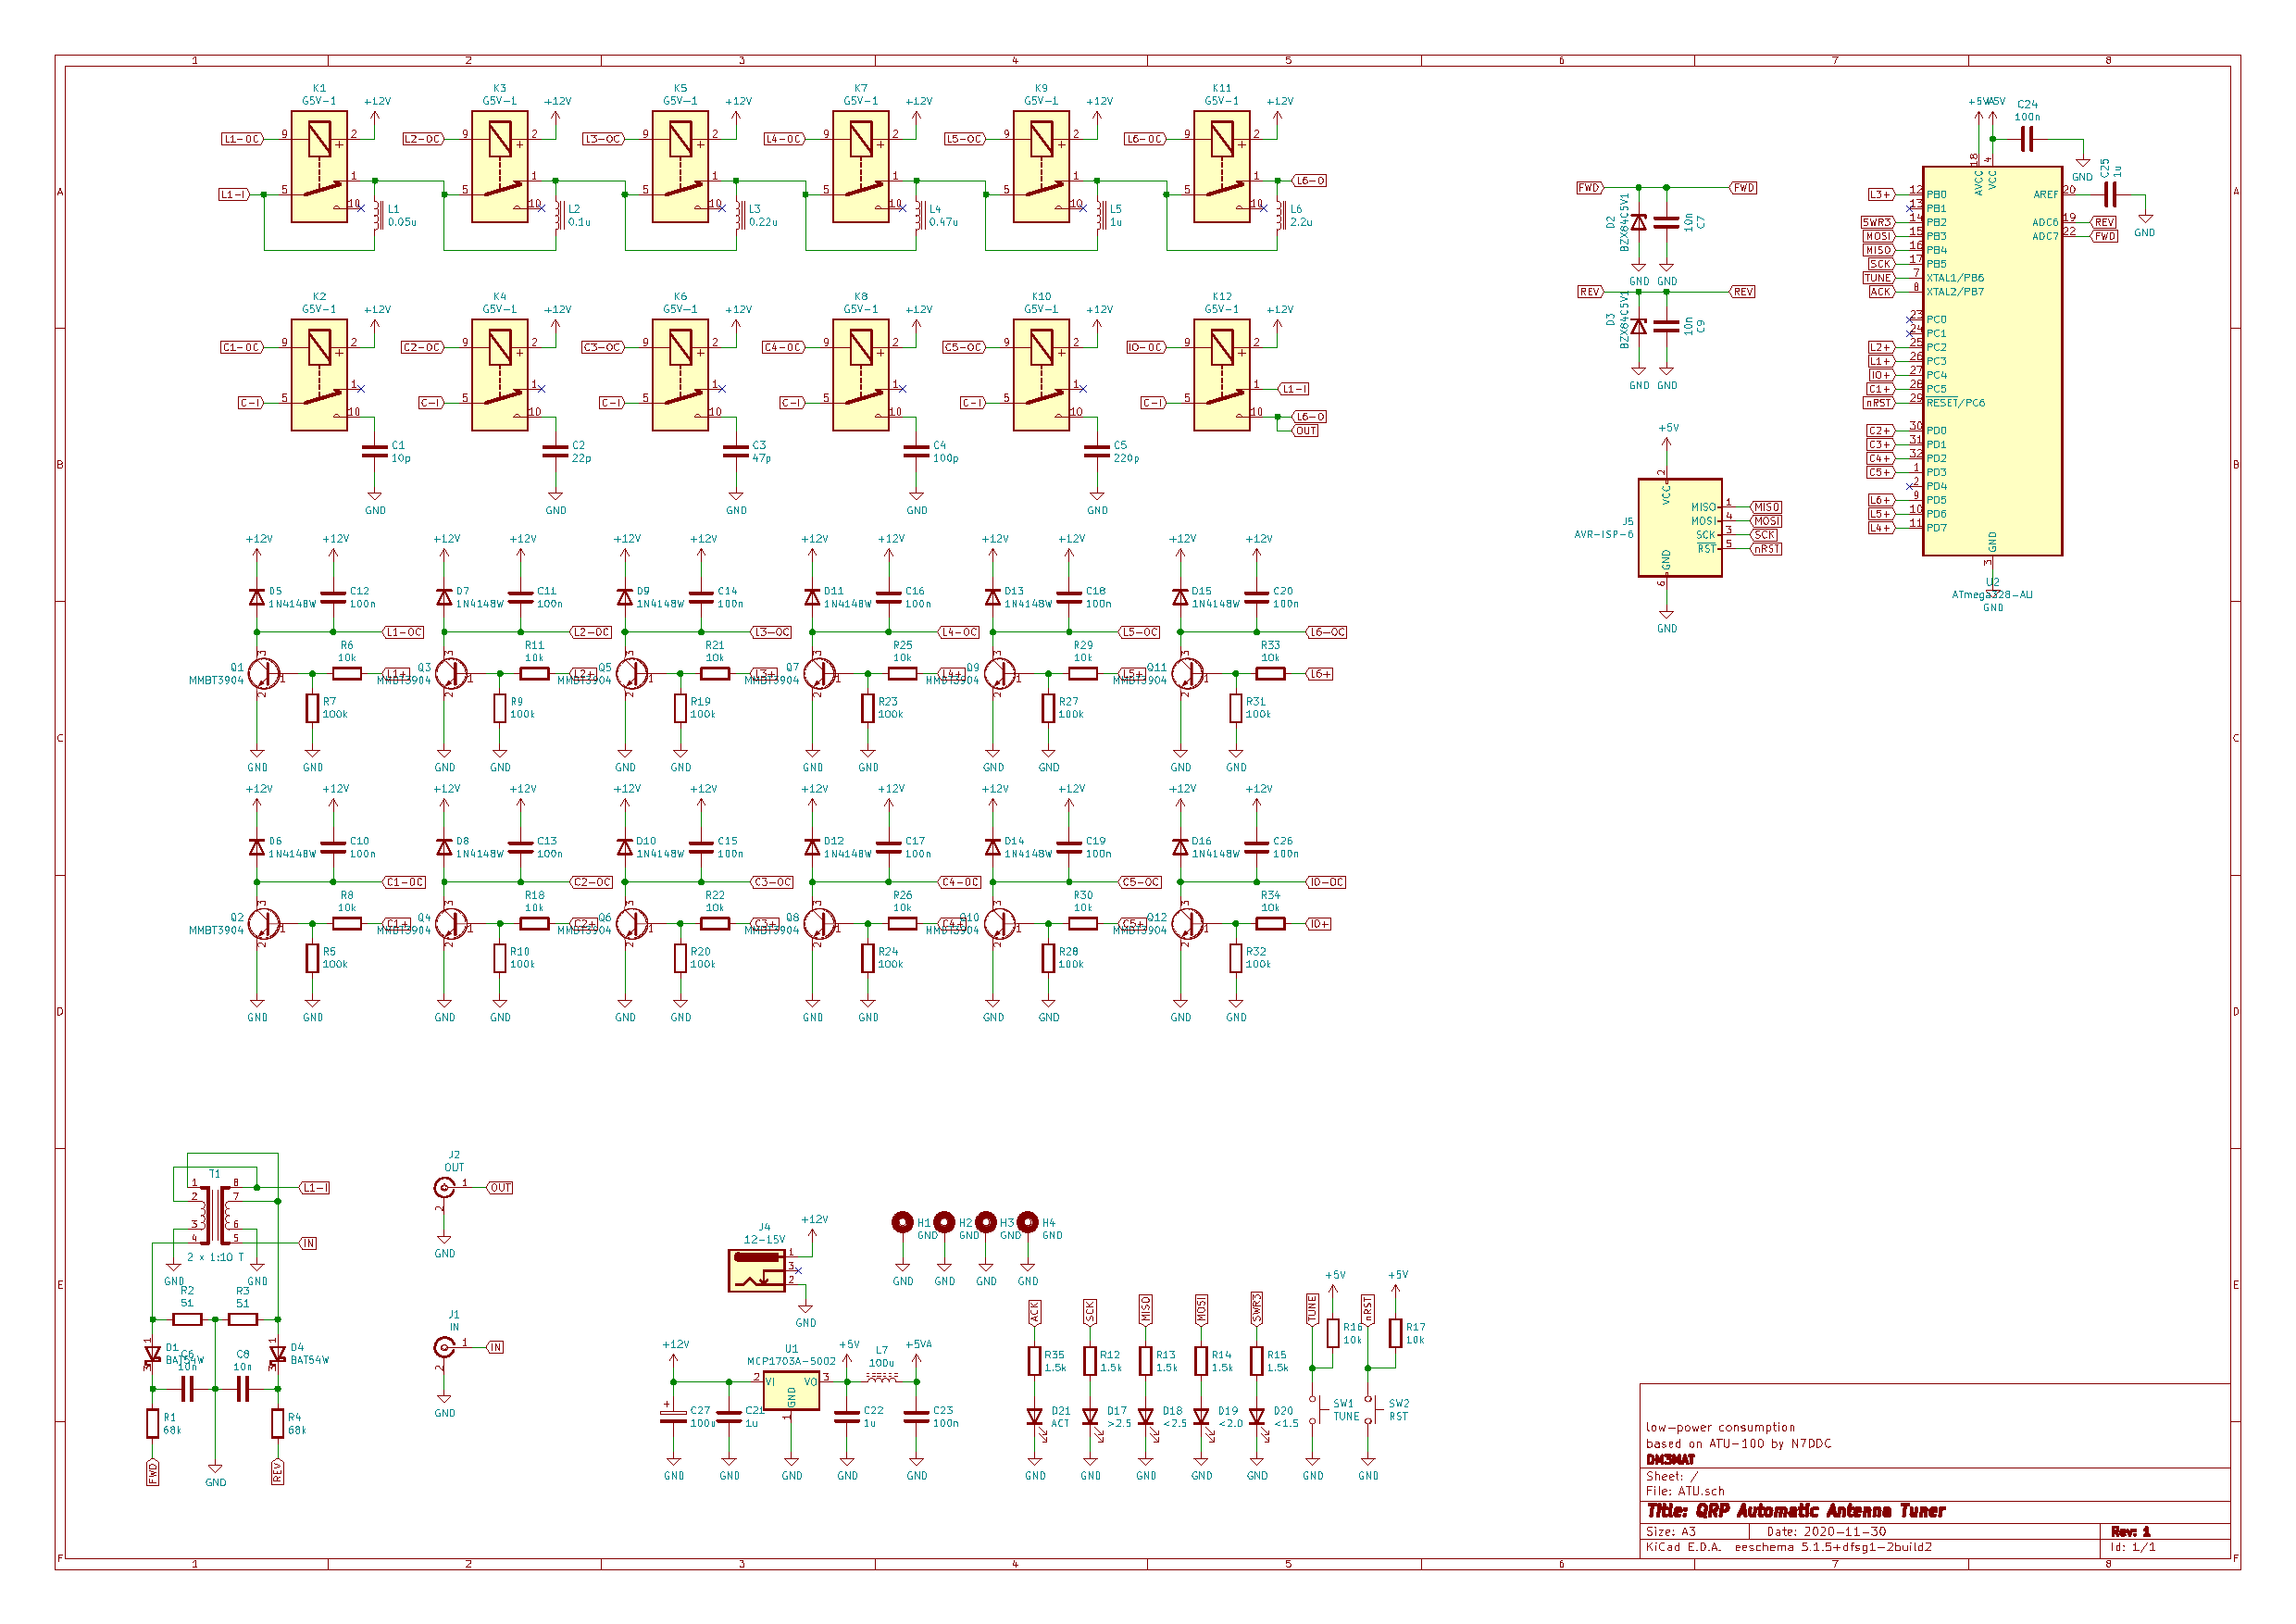
\includepdf[landscape=true, addtotoc={
  1, subsection, 1, Schematic, circuit}]{fig/atu_scm.pdf}


\section{Tuning Algorithm}
Tuning an unknown antenna for an unknown frequency is a relatively difficult task: The VSWR as a function of L and C is certainly not convex. That means, that there are (possibly) many local minima. Finding the best match, that is the global minimum of the VSWR function, gets hard. 

Moreover, the relays take some time to switch and they may bounce after they switched. To this end, a short delay between the signal to switch a relay and the measurement of the current VSWR is needed to get a reliable reading. This delay is in the order of magnitude of about $> 10\,ms$. As many combinations of L's and C's must be tested, the time needed to find a minimum VSWR may get quiet long. Given the 12 relays used in this ATU, the worst-case time to test every possible combination of L's and C's would take at least $41\,s$. 

During this time, the TRX may see high VSWR that may put unbearable stress on the PA transistors. Hence the time needed to find at least a feasible VSWR should be a short as possible. 

Hence, the tuning algorithm tries to find an optimum in two steps. In a first step, a coarse tuning is done by searching a subset of all possible combinations of L and C values for a coarse minimum. This first tuning will likely not achieve the best possible match, but finds a reasonable match very fast.

In a second step, the coarse tuning is refined by fine-tuning L and C alternately until the VSWR cannot be reduced anymore or a sufficiently low VSWR value (e.g., less than 1 : 1.2) is measured.

\subsection{User Manual}
The user-interface is held simple. The front-plate has only two buttons. The left button is the reset button. This button is directly tied to the reset line of the MCU. Pressing this reset button rests the MCU hard and disengages all relays. In this setting the ATU is configured to bypass the signal. 

Pressing the right button, starts the tuning. The left-most LED will start to blink slowly. This signals that the ATU waits for the transmitter to transmit to start the actual tuning. Once sufficient input-power is detected, the tuning starts. In this mode, the left-most LED blinks fast. If no sufficient power gets measured for 5s, the ATU goes back into sleep mode. 

Once the tuning was successful, the ATU will return into sleep mode but maintains the current tuning. If the tuning button is now pressed again, the ATU will fine-tune the current settings again. To discard the current tuning, the reset button must be pressed. This should be done every time the band is changed.

\section{Board \& Electrical Assembly}
The assembly is quiet uncritical. Although there are many SMD parts, they are mainly 1206 resistors and capacitors, which can be hand-soldered easily. A bit more care must be taken for soldering the MCU. The pin-pitch is $0.8\,mm$ and thus is quiet small. However, the pins can still be soldered individually using a fine soldering tip and thin solder. 

\begin{remark}
In general when soldering SMD parts: use plenty of flux. 
\end{remark}

A few parts are soldered on the bottom of the board. This includes the bypass capacitors and shunt diodes for the relays. As the bottom lacks a silk-screen print, please consult the \href{https://dm3mat.darc.de/atu/ATU-ibom.html}{interactive BOM} to get the orientation of the diodes.

The 6 inductors L1--L6 are wound on Amidon iron-powder cores. The following table provides approximate numbers of turns for each coil. 

\begin{center}
\begin{tabular}{|l|l|l|l|} \hline
    & Value & Core  & Turns \\ \hline 
 L1 & 100nH & T44-0 &  \\ 
 L2 & 220nH & T44-0 &  \\ 
 L3 & 470nH & T44-6 &  \\ 
 L4 & 1.0uH & T44-6 &  \\ 
 L5 & 2.2uH & T44-2 &  \\ 
 L6 & 4.7uH & T44-2 &  \\ \hline
\end{tabular}
\end{center}

Remember that every time the wire passes through the core counts as a winding. The given number of turns were obtained using the data-sheet $A_l$-value, hence the number is usually slightly high. Please verify the actual inductance before installing the coil.

\begin{wrapfigure}{o}{.25\linewidth}
 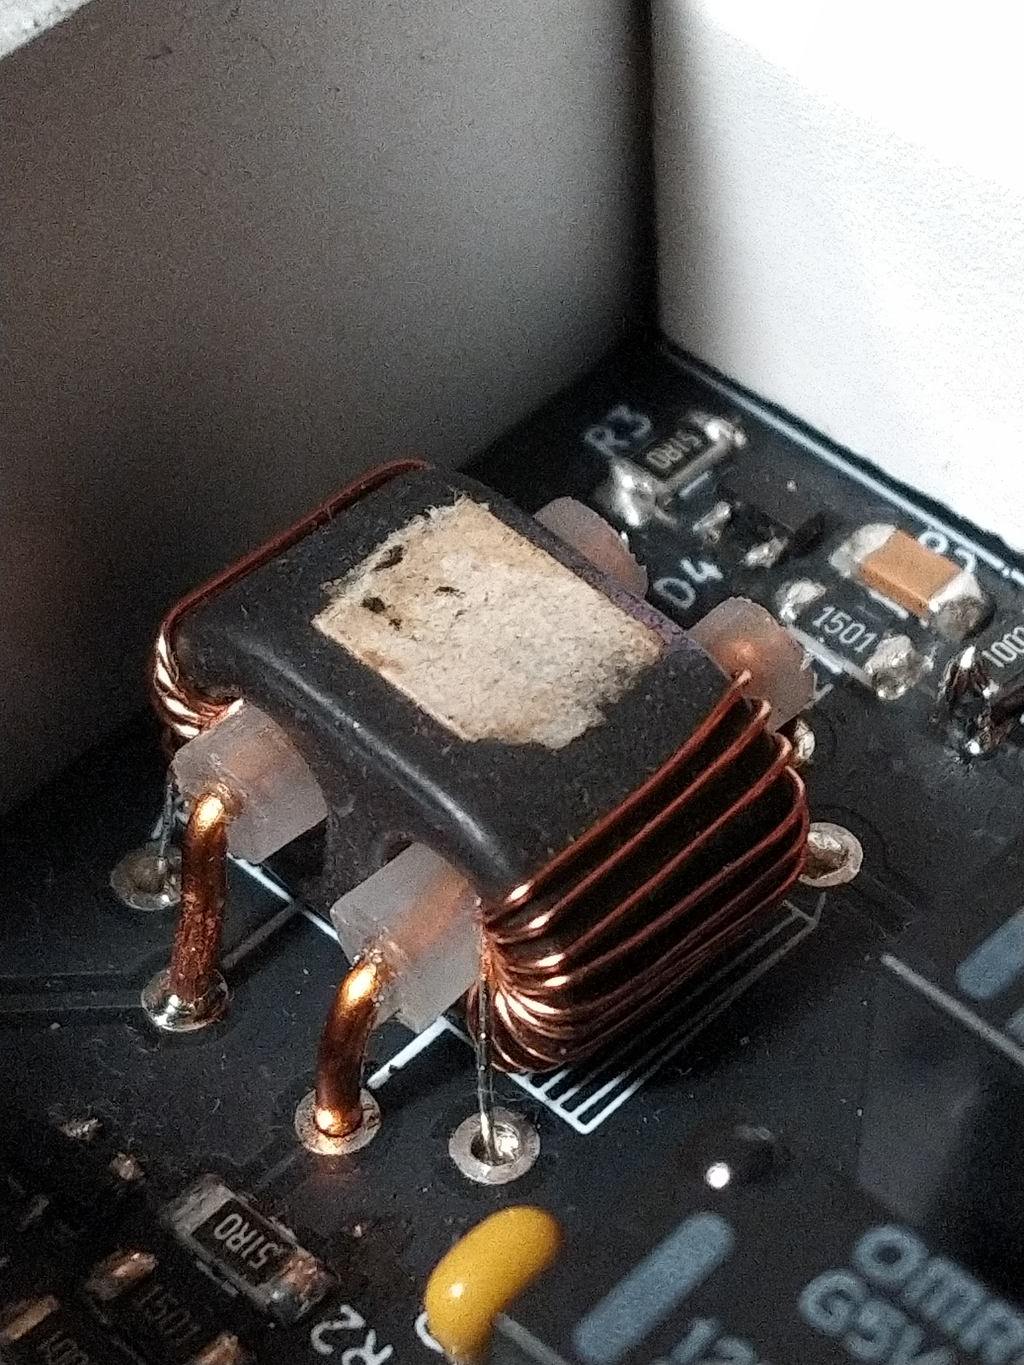
\includegraphics[width=\linewidth]{fig/swr.png}
 \caption{Closeup of the directional coupler.} \label{fig:swr}
\end{wrapfigure}

A bit harder is the winding of the directional coupler. It consists of two current-sense transformer wound on a single binocular ferrite core. These are old TV baluns that can be obtained at swap-meets for almost nothing. The particular one used here, is about $8 \times 14 \times 8\,mm$ in size and of unknown material. 

However, the core and it's material is not that critical as long as the permeability of the material is large enough while keeping the losses small. The common but slightly larger \texttt{BN-42-302} or even better \texttt{BN-62-302} should work as well. The latter has a much smaller permeability and thus should imply much smaller insertion-losses on higher frequencies. The former has a much higher permeability and should be better suited for lower frequencies.

The winding direction of the left and right transformer does not matter. However, they should be the same. The winding-ratio is $1 : 10$. That is, the one primary winding formed by the thick inner wire, implies ten turns on the secondary side. Please note that every time the wire passes though the hole counts as a turn.

The white plastic insulator visible in figure \ref{fig:swr} is not necessary but helps with the mechanical stability of the directional coupler. Two 1cm long pieces of the dielectric material of a RG-58 coax-cable were used here. 

\subsection{Bugs in Revision 0}
\begin{warning}
 There are two 10k resistors missing on the board. They must be installed in parallel to C7 \& C9. As these are G1206 capacitors, these resistors can be installed piggy-back on top of these capacitors.
\end{warning}

\begin{remark}
 The footprint of the Schottky-diodes D1 \& D4 are wrong. They are SOT-323 but should be SOT-23. They are, however, similar enough to still be able to solder the SOT-23 diodes on them. Especially as only two of the three pins are actually needed.
\end{remark}


\section{BOM \& Mechanical Assembly}
The PCB is designed to slide into a small Fischer $10 \times 10 \times 3.2cm$ chassis. All connectors, buttons and LEDs are PCB mounted. Hence, the location of all drill-holes in the front and back-panel are critical. As a drill aid, the locations are shown in figure \ref{front} and \ref{back} below.

The button drill-holes should have a 4mm diameter, for the LEDs use 3.5 diameter holes. The drill-hole for the barrel-jack should have at least 6mm diameter and for the BNC jacks should be $13 mm$ wide and $12mm$ high.  

\clearpage
\subsection{Bill-of-Material}
\begin{longtable}{|p{0.02\textwidth}|p{0.02\textwidth}|p{0.3\textwidth}|p{0.27\textwidth}|p{0.08\textwidth}|p{0.08\textwidth}|}\hline
\# & & Value & Reichelt & Cost & Sum \\ \hline\hline
 2 & $\square$ & 51, SMD 1206 & KOA RK73H2BTTD53 & 0.02 \EUR & 0.04 € \\
 5 & $\square$ & 1.5k, SMD 1206 & RND 1206 1 1,5K & 0.02 \EUR & 0.10 \EUR \\
16 & $\square$ & 10k, SMD 1206 & VIS CRCW120610K & 0.02 \EUR & 0.31 \EUR \\
 2 & $\square$ & 68k, SMD 1206 & RND 1206 1 68K & 0.02 \EUR & 0.04 \EUR \\
12 & $\square$ & 100k, SMD 1206 & VIS CRCW1206100 & 0.02 \EUR & 0.23 \EUR \\ \hline
 1 & $\square$ & 10p, NP0, THT & C3C0G 10p 200 & 0.12 \EUR & 0.12 \EUR \\
 1 & $\square$ & 22p, NP0, THT & C3C0G 22p 200 & 0.12 \EUR & 0.12 \EUR \\
 1 & $\square$ & 47p, NP0, THT & C3C0G 47p 200 & 0.12 \EUR & 0.12 \EUR \\
 1 & $\square$ & 100p, NP0, THT & C3C0G 100p 200 & 0.14 \EUR & 0.14 \EUR \\
 1 & $\square$ & 220p, NP0, THT & C3C0G 220p 200 & 0.15 \EUR & 0.15 \EUR \\
 4 & $\square$ & 10n, SMD 1206 & X7R-G1206 10N & 0.04 \EUR & 0.16 \EUR \\
14 & $\square$ & 100n, SMD 1206 & X7R-G1206 100N & 0.10 \EUR & 1.36 \EUR \\
 3 & $\square$ & 1u, SMD 1206 & KEM X7R1206 1,0U & 0.07 \EUR & 0.21 \EUR \\
 1 & $\square$ & 100u, SMD 6.2x5.8 & ECC ZA160101MF6 & 0.14 \EUR & 0.14 \EUR \\ \hline
 2 & $\square$ & T44-0 & T 44-0 & 0.72 \EUR & 1.44 \EUR \\
 2 & $\square$ & T44-6 & T 44-6 & 0.72 \EUR & 1.44 \EUR \\
 2 & $\square$ & T44-2 & T 44-2 & 0.65 \EUR & 1.30 \EUR \\
 1 & $\square$ & 100u, SMD 1210 & LQH3C 100µ & 0.17 \EUR & 0.17 \EUR \\
 1 & $\square$ & 2 x 1:10 T, binocular & EPCO B62152-A4-X & 0.82 \EUR & 0.82 \EUR \\ \hline
 2 & $\square$ & BAT54W & BAT 54 SMD & 0.05 \EUR & 0.10 \EUR \\
 2 & $\square$ & BZX84C5V1 & BZX 84C5V1 VIS & 0.05 \EUR & 0.10 \EUR \\
12 & $\square$ & 1N4148W & RND 1N4148WS & 0.02 \EUR & 0.23 \EUR \\
 2 & $\square$ & THT, LED 2mA, red & LED 3MM 2MA RT & 0.12 \EUR & 0.24 \EUR \\
 1 & $\square$ & THT, LED, 2mA, yellow & LED 3MM 2MA GE & 0.12 \EUR & 0.12 \EUR \\
 2 & $\square$ & THT, LED, 2mA, green & LED 3MM 2MA GN & 0.12 \EUR & 0.24 \EUR \\
12 & $\square$ & MMBT3904 & MMBT 3904LT1G & 0.03 \EUR & 0.36 \EUR \\
 1 & $\square$ & MCP1703A-5002 & MCP 1703A-5002 & 0.58 \EUR & 0.58 \EUR \\
 1 & $\square$ & ATMega328P-AU & ATMEGA 328P-AU & 1.94 \EUR & 1.94 \EUR \\ \hline
12 & $\square$ & G5V-1 12V & G5V-1 12V & 0.88 \EUR & 10.56 \EUR \\
 2 & $\square$ & Push-button, 90deg & TASTER 3305B & 0.20 \EUR & 0.40 \EUR \\
 2 & $\square$ & BNC Connector & UG 1094W1 & 1.00 \EUR & 2.00 \EUR \\
 1 & $\square$ & Barrel Connector & DC BU21 90 & 0.46 \EUR & 0.46 \EUR \\
 1 & $\square$ & AVR-ISP-6 & MPE 087-2-006 & 0.14 \EUR & 0.14 \EUR \\ 
 2 & $\square$ & Fisher Chasis & KOH-1100 & 5.12 \EUR & 10.24 \EUR \\
 1 & $\square$ & Front + Back & DPL 1-1 & 6.43 \EUR & 6.43 \EUR \\ \hline \hline
   & & & & Total & 41.53 \EUR \\ \hline
\end{longtable}


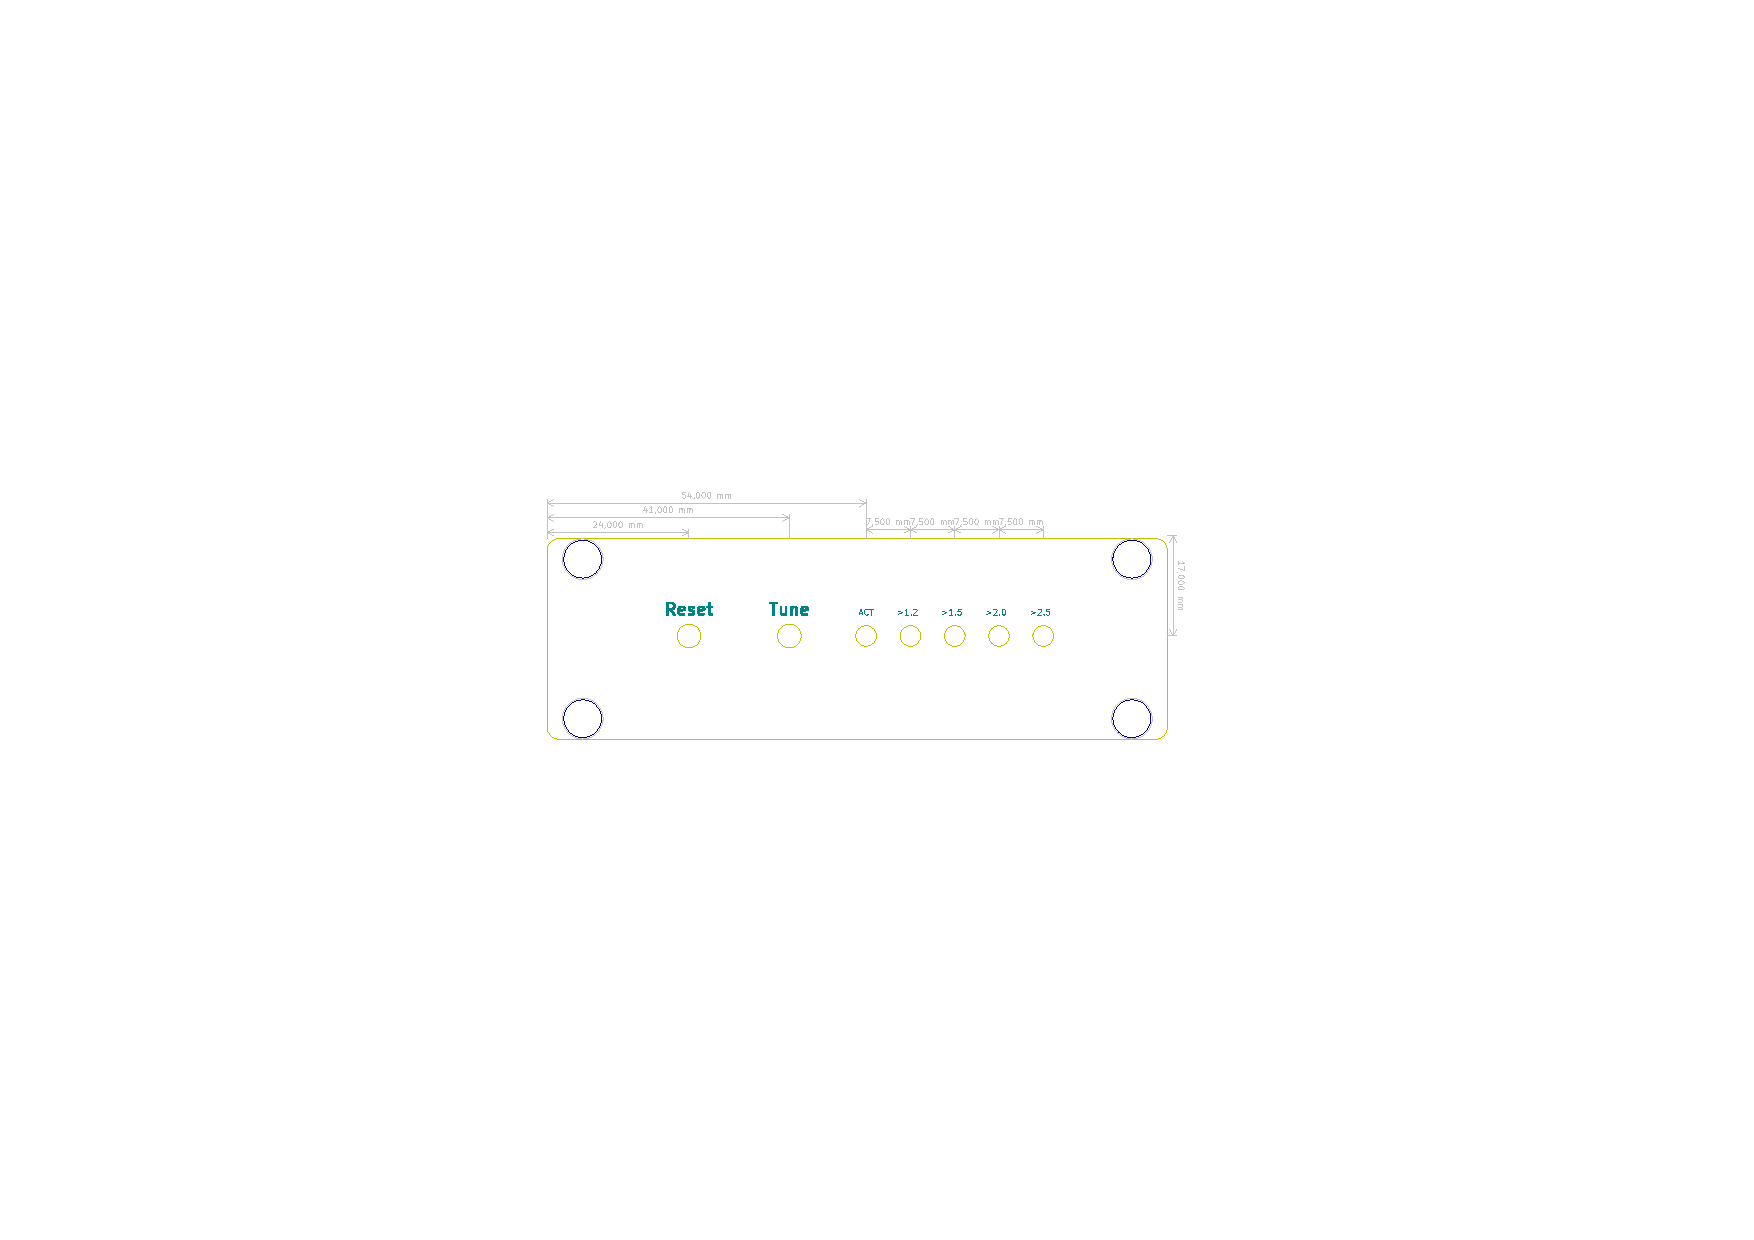
\includepdf[landscape=true, fitpaper=false, addtotoc={
  1, subsection, 1, Frontplate, front}]{fig/front.pdf}
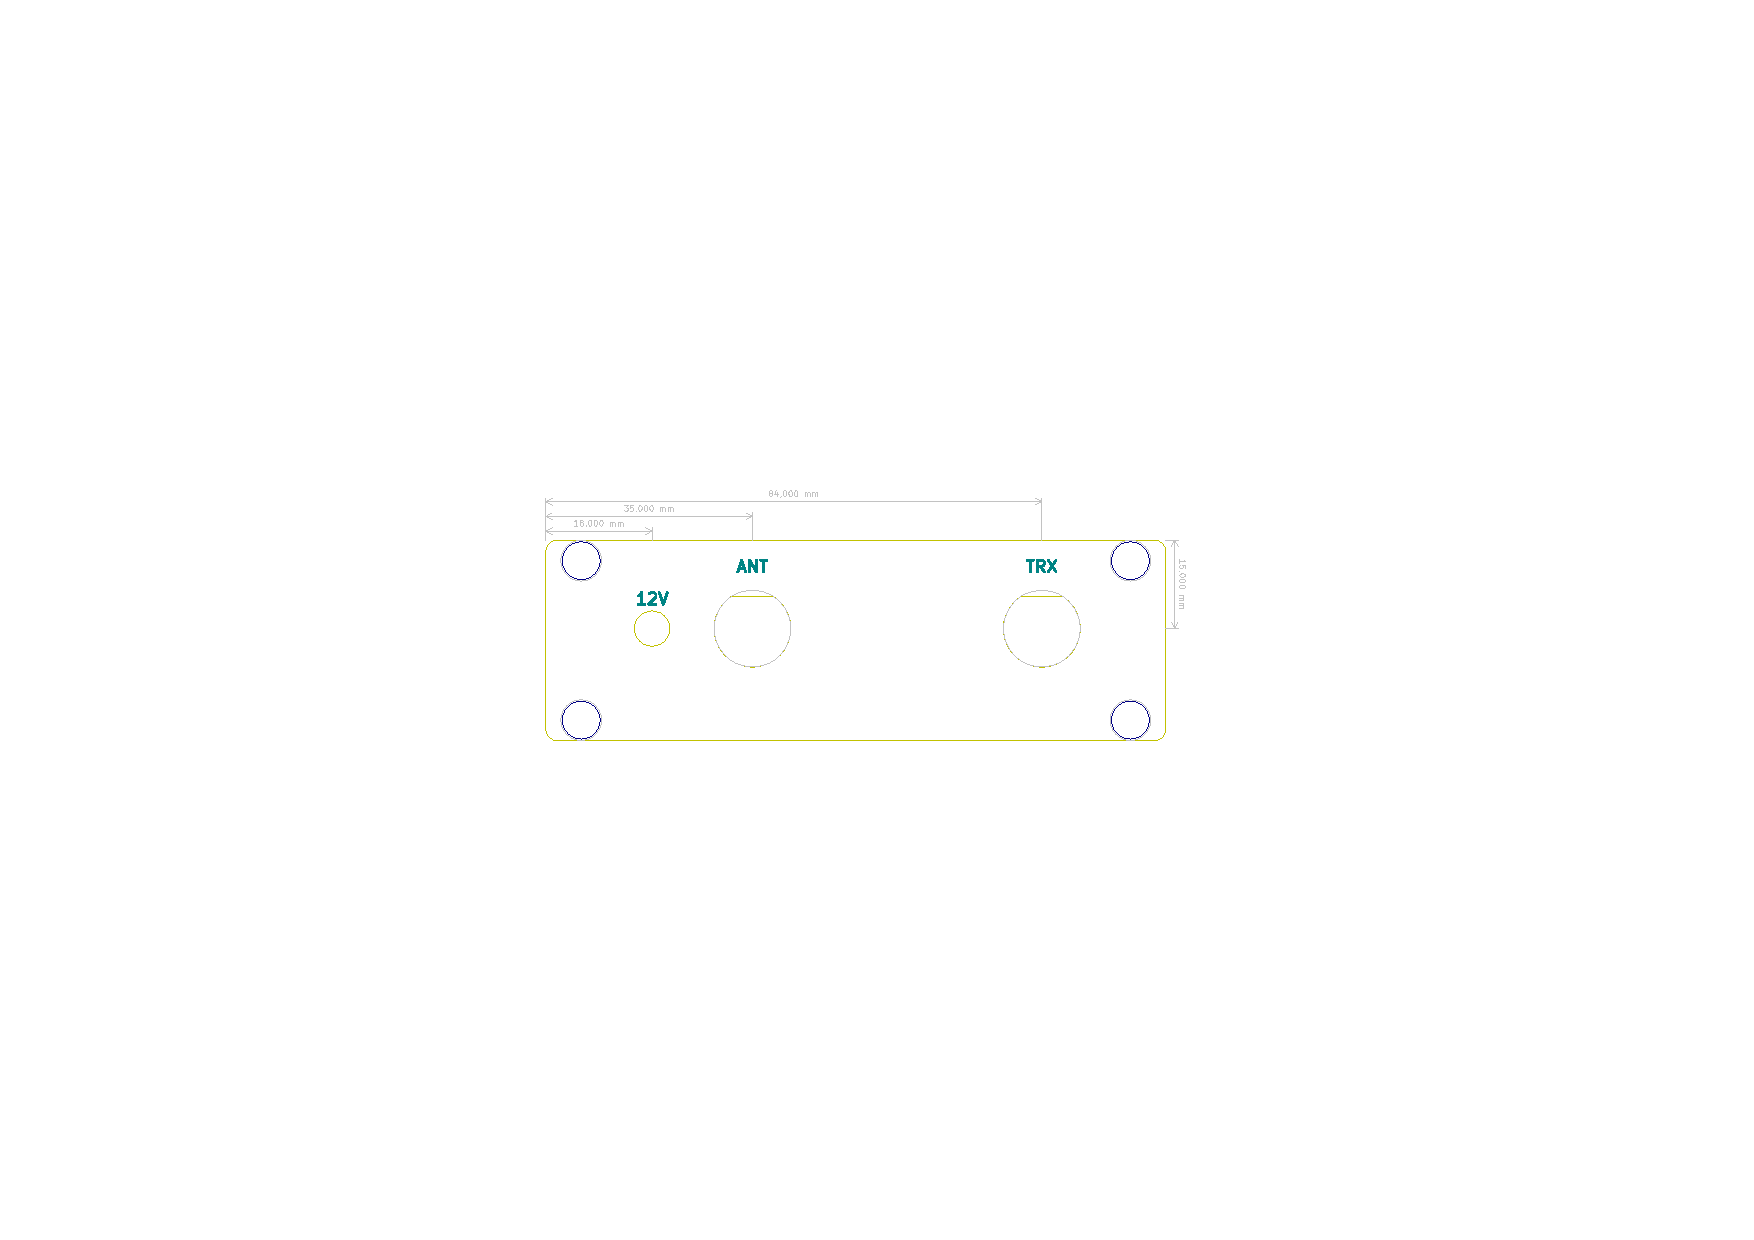
\includepdf[landscape=true, fitpaper=false, addtotoc={
  1, subsection, 1, Backplate, back}]{fig/back.pdf}

\end{document}